\documentclass[12pt]{article}
\usepackage[margin=2cm]{geometry}
\usepackage{titling}
\usepackage[T1]{fontenc}
\usepackage{tabularx}
\usepackage{graphicx}
\usepackage{subcaption}
\usepackage{amsfonts}
\usepackage{amsmath}
\usepackage{amssymb}
\usepackage{algorithm}
\usepackage[noend]{algpseudocode}

\pretitle{\begin{center}\Huge\bfseries}
\posttitle{\par\end{center}\vskip 0.5em}
\preauthor{\begin{center}\Large}
\postauthor{\end{center}}
\predate{\par\large\centering}
\postdate{\par}

\title{Algorytmy Metaheurystyczne - lab 2}
\author{Jakub Musiał 268442}
\date{Listopad 2023}

\begin{document}

\maketitle

\vspace*{2cm}

\section{Opis problemu}
Wyznaczyć cykl komiwojażera dla grafu pełnego używając algorytmów \textit{Simulated Annealing} oraz
\textit{Taboo Search}.
\noindent\newline
W implementacji algorytmów stosowałem otoczenie \textit{invert}:
$$N(\pi) = \{\pi' \in S(P) : (\exists \text{ } i \ne j)(\pi' = invert(\pi, i, j))\}$$
gdzie $P$ - wejściowy zbiór punktów.

\section{Symulowane wyżarzanie}
    \subsection{Dobór parametrów}
        By określić najlepsze parametry przeprowadziłem eksperyment polegający na sprawdzeniu wyników
        kombinacji z losowej próbki wszystkich możliwych kombinacji poniżej określonych parametrów,
        a następnie znajdując taką, która generuje najmniejszy błąd względny.
        \newline

        \noindent \textbf{Badane parametry:}
        \begin{itemize}
            \item $T_0$ - temperatura początkowa: $\{10, 50, 100\}$
            \item $T_k$ - temperatura minimalna: $\{0.9, 0.95, 0.99\}$
            \item $\alpha$ - współczynnik zmiany temperatury: $\{0.01, 0.1, 1.0\}$
            \item $it_{max}$ - maxymalna liczba iteracji (jako procent liczby wierzchołków grafu): $\{0.1, 0.2, 0.3\}$
        \end{itemize}

        \noindent Najlepszą znalezioną kombinacją parametrów jest:
        $T_0 = 100$, $T_k = 0.1$, $\alpha = 0.99$, $it_{max} = 0.3$,
        dla której otrzymałem następujące wyniki:

    \newpage

        \begin{table}[h!]
        \centering
        \begin{tabularx}{0.4225\textwidth}{| c | c | c |}
            \hline
            Dane wejściowe & $min_{c}(\delta{w})$ & $avg_{c}(\delta{w})$ \\
            \hline
            xqf131 & $0.000000$ & $0.015957$ \\
            xqg237 & $0.003925$ & $0.019627$ \\
            pma343 & $0.002924$ & $0.006579$ \\
            pka379 & $0.004505$ & $0.008258$ \\
            bcl380 & $0.016656$ & $0.025293$ \\
            pbl395 & $0.014052$ & $0.018735$ \\
            pbk411 & $0.009680$ & $0.022338$ \\
            pbn423 & $0.004396$ & $0.024908$ \\
            pbm436 & $0.018018$ & $0.024255$ \\
            xql662 & $0.015519$ & $0.02865$ \\
            \hline
        \end{tabularx}
        \label{table:sa_exp}
        \caption{Wyniki eksperymentów dla algorytmu symulowanego wyżarzania}
        \end{table}

    \noindent\newline

    \subsection{Pseudokod algorytmu}

        \begin{algorithm}[h!]
        \caption{Symulowane wyżarzanie}\label{alg:simulated_annealing}
        \begin{algorithmic}[1]
            \Procedure{$simulated\_annealing$}{$\pi_0$}
                \State $\pi_b \gets \pi_0$
                    \Comment Best permutation
                \State $T \gets T_0$
                \State
                \While{$T > T_k$}
                    \State $\pi \gets \pi_b$
                    \State $(i, j) \gets (0, 0)$
                    \State
                    \While{$it < it_{max}$}
                        \State $(i, j) \gets random\_element(N(\pi))$
                        \State $\Delta{w} \gets invert\_wdiff(\pi, i, j)$
                        \If{$\Delta{w} < 0 \lor random\_prob() < e^{\frac{-\Delta{w}}{T}}$}
                            \State $invert(\pi, i, j)$
                            \State $it \gets it + 1$
                            \If{$w(\pi) < w(\pi_b)$}
                                \State $\pi_b \gets \pi$
                            \EndIf
                        \EndIf
                    \EndWhile
                    \State $T \gets \alpha T$
                \EndWhile
                \State
                \Return $\pi_b$
            \EndProcedure
        \end{algorithmic}
        \end{algorithm}

    \newpage

    \subsection{Wyniki}
        Poniższa tabela oraz wykresy przedstawiają wyniki uzyskane dla wszystkich grafów testowych dla
        znalezionej kombinacji parametrów.

        \begin{table}[h!]
        \centering
        \begin{tabularx}{0.91\textwidth}{| c | c | c | c | c | c |}
            \hline
            Dane wejściowe & $|V|$ & $avg(w(TSC))$ & $min(w(TSC))$ & $w(TSC_{opt})$ & $avg_{ls}(w(TSC))$ \\
            \hline
            xqf131.tsp  & $131$  & $576$  & $569$  & $564$  & $621$ \\
            xqg237.tsp  & $237$  & $1049$ & $1031$ & $1019$ & $1118$ \\
            pma343.tsp  & $343$  & $1380$ & $1372$ & $1368$ & $1497$ \\
            pka379.tsp  & $379$  & $1341$ & $1333$ & $1332$ & $1450$ \\
            bcl380.tsp  & $380$  & $1663$ & $1635$ & $1621$ & $1817$ \\
            pbl395.tsp  & $395$  & $1312$ & $1296$ & $1281$ & $1456$ \\
            pbk411.tsp  & $411$  & $1380$ & $1362$ & $1343$ & $1489$ \\
            pbn423.tsp  & $423$  & $1403$ & $1385$ & $1365$ & $1533$ \\
            pbm436.tsp  & $436$  & $1481$ & $1470$ & $1443$ & $1629$ \\
            xql662.tsp  & $662$  & $2583$ & $2567$ & $2513$ & $2822$ \\
            xit1083.tsp & $1083$ & $3655$ & $3621$ & $3558$ & $4021$ \\
            icw1483.tsp & $1483$ & $4532$ & $4506$ & $4416$ & $4986$ \\
            djc1785.tsp & $1785$ & $6273$ & $6244$ & $6115$ & $6878$ \\
            dcb2086.tsp & $2086$ & $6810$ & $6776$ & $6600$ & $7463$ \\
            pds2566.tsp & $2566$ & $7898$ & $7861$ & -      & $8695$ \\
            \hline
        \end{tabularx}
        \label{table:sa_result}
        \caption{Wyniki dla wszystkich danych wejściowych dla algorytmu symulowanego wyżarzania wraz z
        wagą optymalnych ścieżek oraz wynikami algorytmu local search z listy 1}
        \end{table}

        \noindent\newline

        \begin{figure}[htpb]
        \centering
            \begin{subfigure}[b]{0.475\textwidth}
                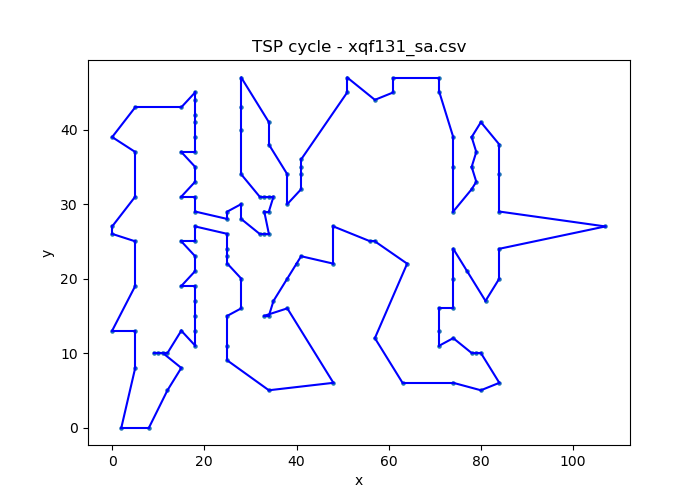
\includegraphics[width=\linewidth]{img/xqf131_sa.png}
            \end{subfigure}
            \hfill
            \begin{subfigure}[b]{0.475\textwidth}
                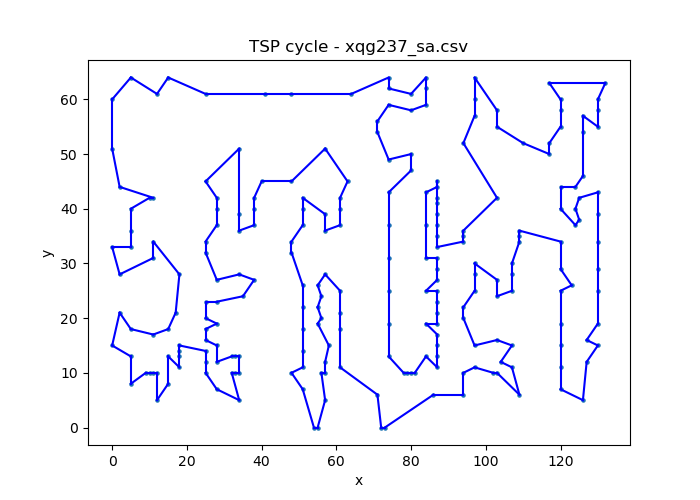
\includegraphics[width=\linewidth]{img/xqg237_sa.png}
            \end{subfigure}
        \end{figure}

        \begin{figure}[htpb]
        \centering
            \begin{subfigure}[b]{0.475\textwidth}
                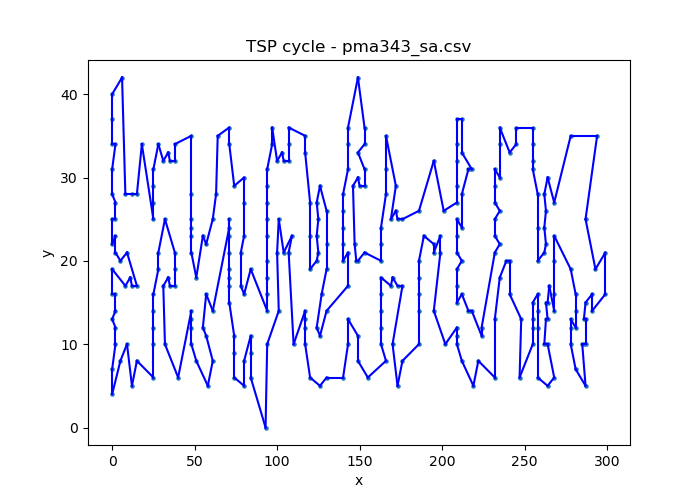
\includegraphics[width=\linewidth]{img/pma343_sa.png}
            \end{subfigure}
            \hfill
            \begin{subfigure}[b]{0.475\textwidth}
                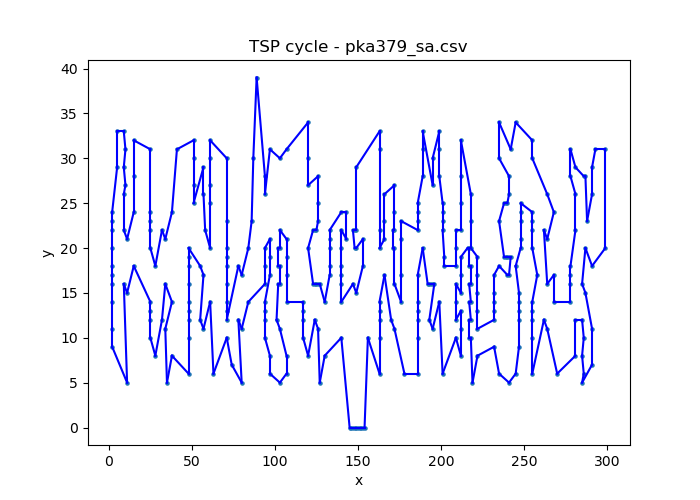
\includegraphics[width=\linewidth]{img/pka379_sa.png}
            \end{subfigure}
            \begin{subfigure}[b]{0.475\textwidth}
                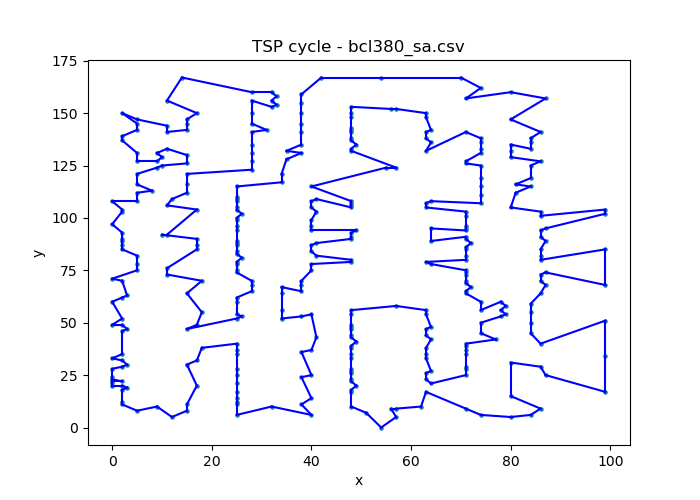
\includegraphics[width=\linewidth]{img/bcl380_sa.png}
            \end{subfigure}
            \hfill
            \begin{subfigure}[b]{0.475\textwidth}
                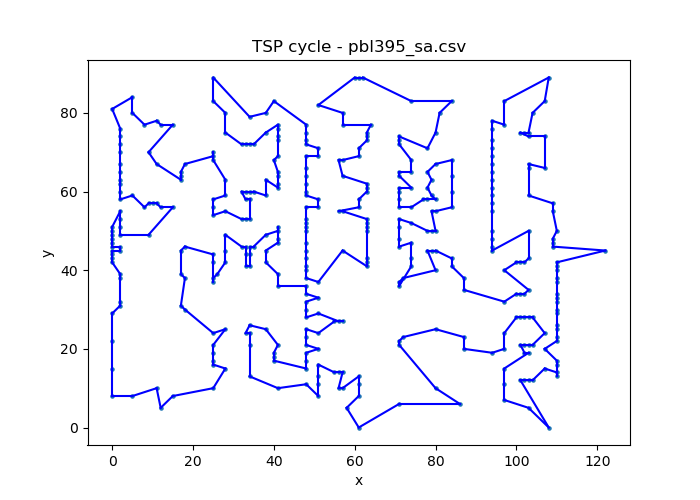
\includegraphics[width=\linewidth]{img/pbl395_sa.png}
            \end{subfigure}
            \begin{subfigure}[b]{0.475\textwidth}
                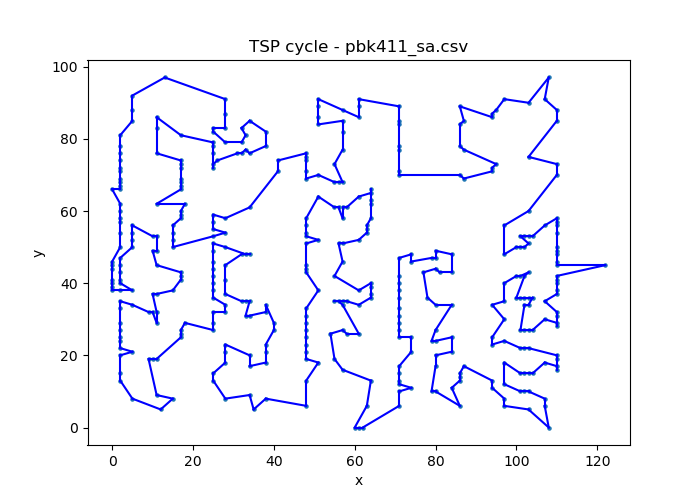
\includegraphics[width=\linewidth]{img/pbk411_sa.png}
            \end{subfigure}
            \hfill
            \begin{subfigure}[b]{0.475\textwidth}
                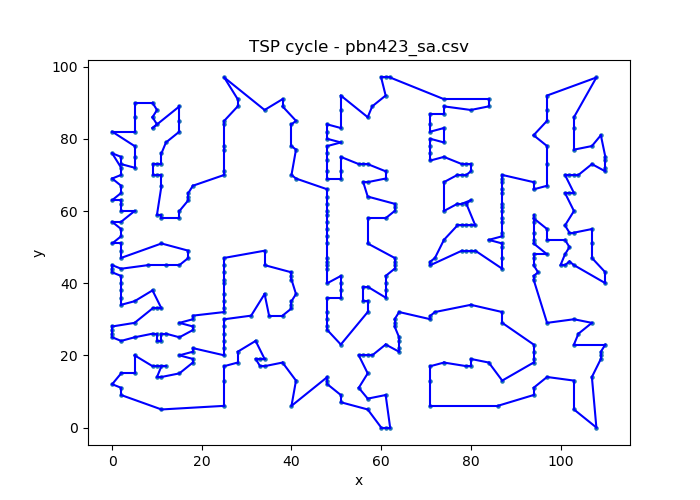
\includegraphics[width=\linewidth]{img/pbn423_sa.png}
            \end{subfigure}
            \centering
            \begin{subfigure}[b]{0.475\textwidth}
                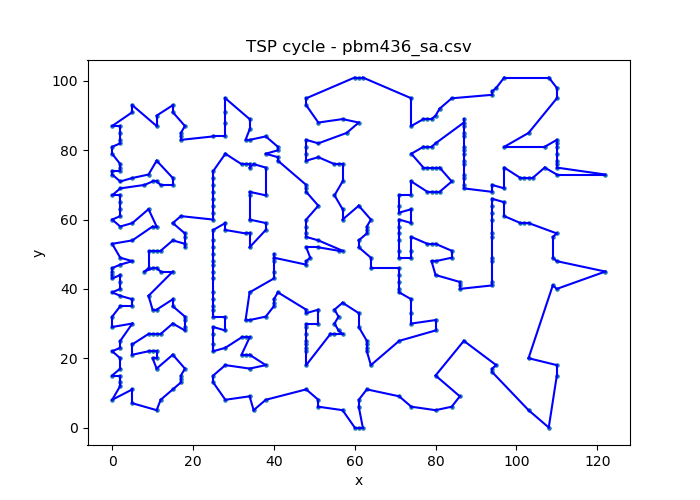
\includegraphics[width=\linewidth]{img/pbm436_sa.png}
            \end{subfigure}
            \hfill
            \begin{subfigure}[b]{0.475\textwidth}
                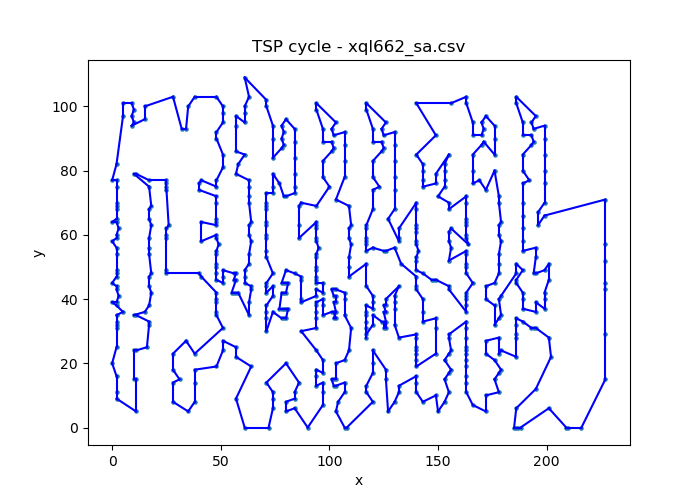
\includegraphics[width=\linewidth]{img/xql662_sa.png}
            \end{subfigure}
        \end{figure}

        \begin{figure}[htpb]
            \begin{subfigure}[b]{0.475\textwidth}
                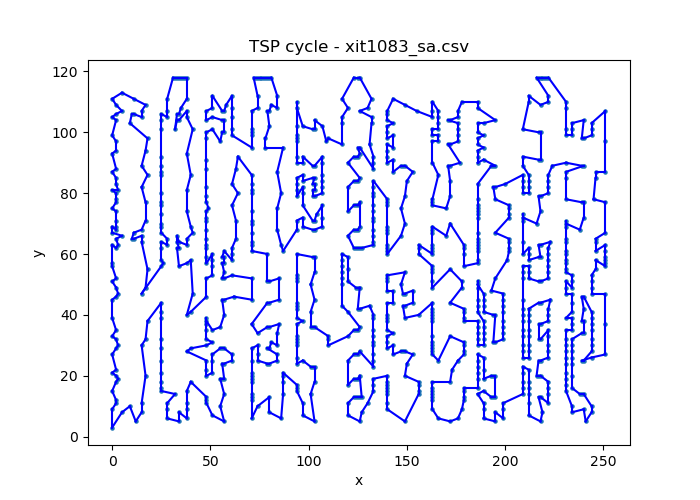
\includegraphics[width=\linewidth]{img/xit1083_sa.png}
            \end{subfigure}
            \hfill
            \begin{subfigure}[b]{0.475\textwidth}
                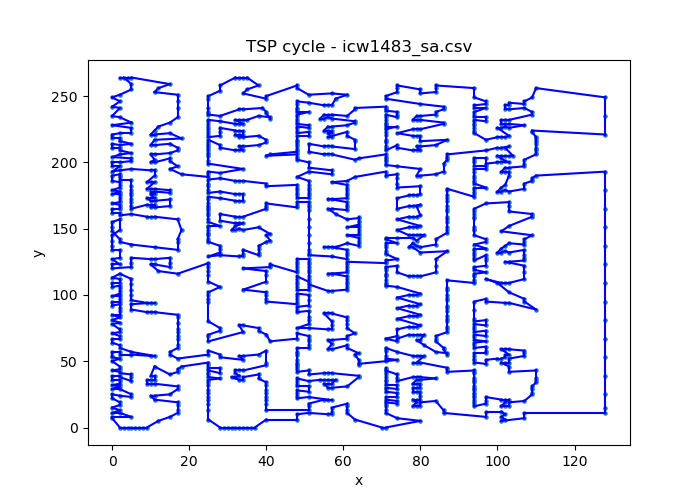
\includegraphics[width=\linewidth]{img/icw1483_sa.png}
            \end{subfigure}
            \begin{subfigure}[b]{0.475\textwidth}
                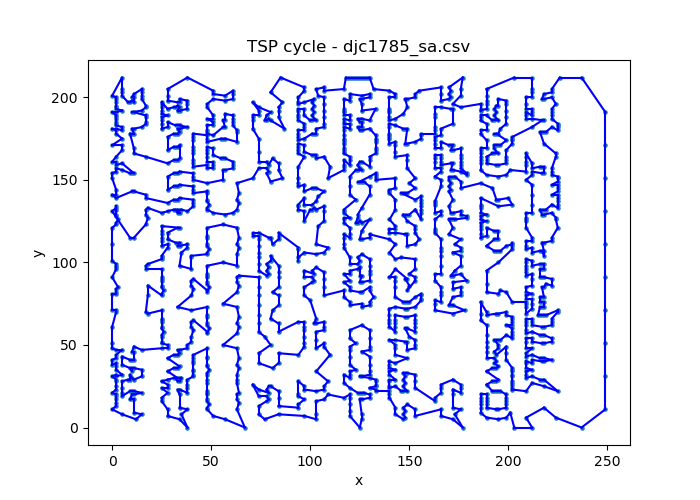
\includegraphics[width=\linewidth]{img/djc1785_sa.png}
            \end{subfigure}
            \hfill
            \begin{subfigure}[b]{0.475\textwidth}
                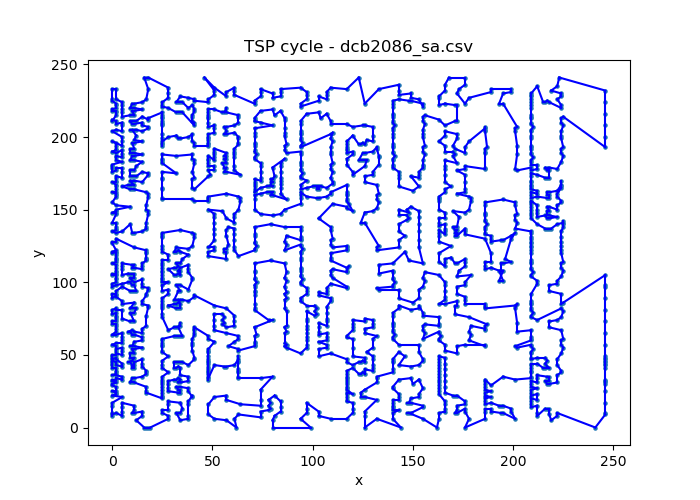
\includegraphics[width=\linewidth]{img/dcb2086_sa.png}
            \end{subfigure}
            \begin{subfigure}[b]{0.475\textwidth}
                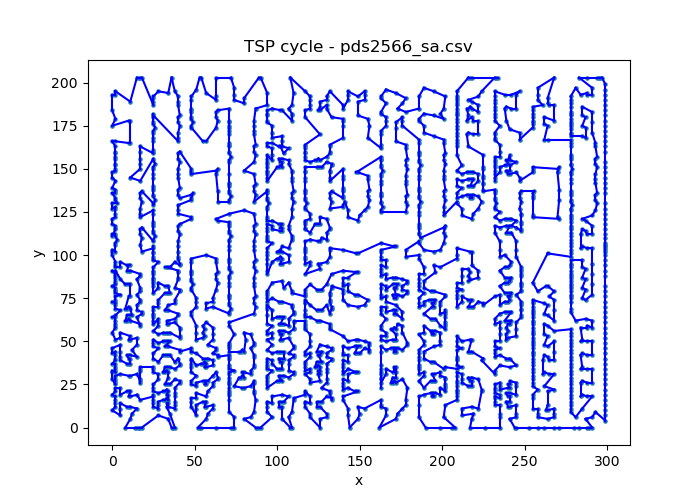
\includegraphics[width=\linewidth]{img/pds2566_sa.png}
            \end{subfigure}
            \caption{Symulowanego wyżarzanie: wizualizacja wyznaczonych cykli komiwojażera}
        \end{figure}

    \newpage

\section{Taboo search}
    \subsection{Dobór parametrów}
        By określić najlepsze parametry przeprowadziłem eksperyment polegający na sprawdzeniu wyników
        wszystkich możliwych kombinacji poniżej określonych parametrów, a następnie znajdując taką,
        która generuje najmniejszy błąd względny.
        \newline

        \noindent \textbf{Badane parametry:}
        \begin{itemize}
            \item $S_{max}$ - maksymalny rozmiar listy wykluczeń: $\{10, 20, 50, 100\}$
            \item $it_{max}$ - maxymalna liczba iteracji bez poprawy rozwiązania: $\{5, 10, 20, 50\}$
        \end{itemize}

        \noindent\newline Najlepszą znalezioną kombinacją parametrów jest: $S_{max} = 100$, $it_{max} = 5$

        \begin{table}[h!]
        \centering
        \begin{tabularx}{0.4225\textwidth}{| c | c | c |}
            \hline
            Dane wejściowe & $min_{c}(\delta{w})$ & $avg_{c}(\delta{w})$ \\
            \hline
            xqf131 & $0.023050$ & $0.079787$ \\
            xqg237 & $0.067713$ & $0.098135$ \\
            pma343 & $0.070906$ & $0.070906$ \\
            pka379 & $0.054054$ & $0.084835$ \\
            bcl380 & $0.080814$ & $0.104874$ \\
            pbl395 & $0.096019$ & $0.117096$ \\
            pbk411 & $0.097543$ & $0.107223$ \\
            pbn423 & $0.090842$ & $0.112821$ \\
            pbm436 & $0.082467$ & $0.119889$ \\
            xql662 & $0.095901$ & $0.126940$ \\
            \hline
        \end{tabularx}
        \label{table:ts_exp}
        \caption{Wyniki eksperymentów dla algorytmu taboo search}
        \end{table}

    \newpage

    \subsection{Pseudokod algorytmu}

        \begin{algorithm}[h!]
            \caption{Taboo search}\label{alg:taboo_search}
            \begin{algorithmic}[1]
                \Procedure{$simulated\_annealing$}{$\pi_0$}
                    \State $\pi_b \gets \pi_0$
                        \Comment Best permutation
                    \State $T \gets \{\}$
                        \Comment Taboo list
                    \State $it \gets 0$
                        \Comment Number of iterations without updating the result
                    \State
                    \While{$it < it_{max}$}
                        \State $\pi \gets \pi_b$
                        \State $w_{bc} \gets \infty$
                            \Comment Best candidate weight
                        \State $(i_b, j_b) \gets null$
                        \State
                        \For{$(i, j) \in N(\pi)$}
                            \State $\Delta{w} \gets invert\_wdiff(\pi, i, j)$
                            \If{$\Delta{w} \geq 0 \land (i, j) \in T \land$}
                                \State \textbf{continue}
                            \EndIf
                            \If{$w(\pi) + \Delta{w} < w_{bc}$}
                                \State $(i_b, j_b) \gets (i, j)$
                                \State $w_{bc} \gets w(\pi) + \Delta{w}$
                            \EndIf
                        \EndFor
                        \State
                        \State $push(T, (i_b, j_b))$
                        \If{$|T| > T_{mp}$}
                            \State $remove\_first(T)$
                        \EndIf
                        \State
                        \If{$w_{bc} < w(\pi_b)$}
                            \State $invert(\pi_b, i_b, j_b)$
                            \State $it \gets 0$
                        \EndIf
                    \EndWhile
                    \State
                    \Return $\pi_b$
                \EndProcedure
            \end{algorithmic}
            \end{algorithm}

    \newpage

    \subsection{Wyniki}
        Poniższa tabela oraz wykresy przedstawiają wyniki uzyskane dla wszystkich grafów testowych dla
        znalezionej kombinacji parametrów.

        \begin{table}[h!]
        \centering
        \begin{tabularx}{0.91\textwidth}{| c | c | c | c | c | c |}
            \hline
            Dane wejściowe & $|V|$ & $avg(w(TSC))$ & $min(w(TSC))$ & $w(TSC_{opt})$ & $avg_{ls}(w(TSC))$ \\
            \hline
            xqf131.tsp  & $131$  & $614$  & $586$  & $564$  & $621$ \\
            xqg237.tsp  & $237$  & $1108$ & $1076$ & $1019$ & $1118$ \\
            pma343.tsp  & $343$  & $1485$ & $1452$ & $1368$ & $1497$ \\
            pka379.tsp  & $379$  & $1447$ & $1423$ & $1332$ & $1450$ \\
            bcl380.tsp  & $380$  & $1802$ & $1770$ & $1621$ & $1817$ \\
            pbl395.tsp  & $395$  & $1431$ & $1395$ & $1281$ & $1456$ \\
            pbk411.tsp  & $411$  & $1485$ & $1444$ & $1343$ & $1489$ \\
            pbn423.tsp  & $423$  & $1528$ & $1510$ & $1365$ & $1533$ \\
            pbm436.tsp  & $436$  & $1611$ & $1571$ & $1443$ & $1629$ \\
            xql662.tsp  & $662$  & $2816$ & $2779$ & $2513$ & $2822$ \\
            xit1083.tsp & $1083$ & $3936$ & $3976$ & $3558$ & $4021$ \\
            icw1483.tsp & $1483$ & $4886$ & $4885$ & $4416$ & $4986$ \\
            djc1785.tsp & $1785$ & $6837$ & $6820$ & $6115$ & $6878$ \\
            dcb2086.tsp & $2086$ & $7342$ & $7329$ & $6600$ & $7463$ \\
            pds2566.tsp & $2566$ & $8685$ & $8622$ & -      & $8695$ \\
            \hline
        \end{tabularx}
        \label{table:ts_result}
        \caption{Wyniki dla wszystkich danych wejściowych dla algorytmu symulowanego wyżarzania wraz z
        wagą optymalnych ścieżek oraz wynikami algorytmu local search z listy 1}
        \end{table}

        \noindent\newline

        \begin{figure}[htpb]
        \centering
            \begin{subfigure}[b]{0.475\textwidth}
                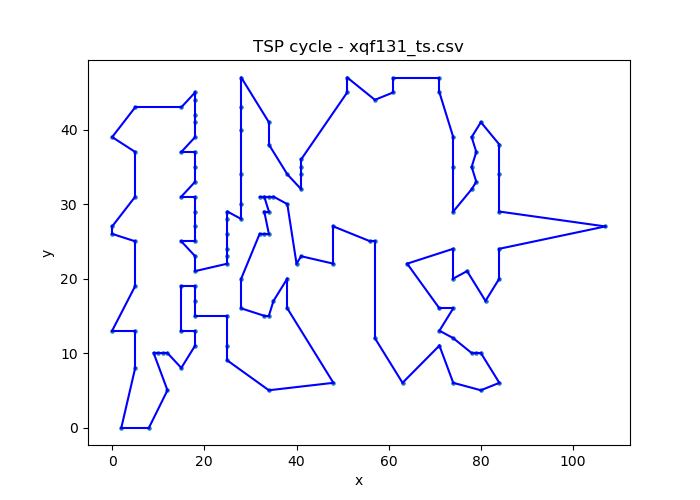
\includegraphics[width=\linewidth]{img/xqf131_ts.png}
            \end{subfigure}
            \hfill
            \begin{subfigure}[b]{0.475\textwidth}
                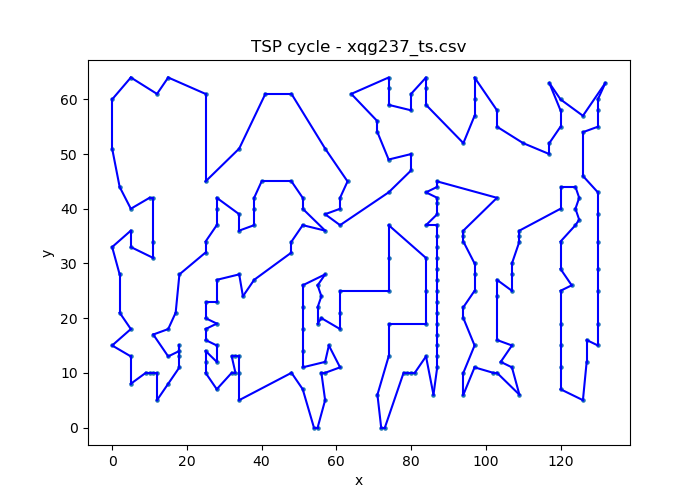
\includegraphics[width=\linewidth]{img/xqg237_ts.png}
            \end{subfigure}
        \end{figure}

        \begin{figure}[htpb]
        \centering
            \begin{subfigure}[b]{0.475\textwidth}
                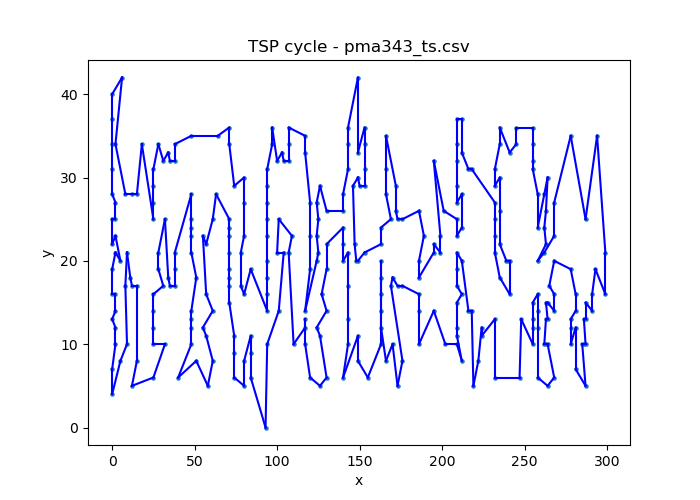
\includegraphics[width=\linewidth]{img/pma343_ts.png}
            \end{subfigure}
            \hfill
            \begin{subfigure}[b]{0.475\textwidth}
                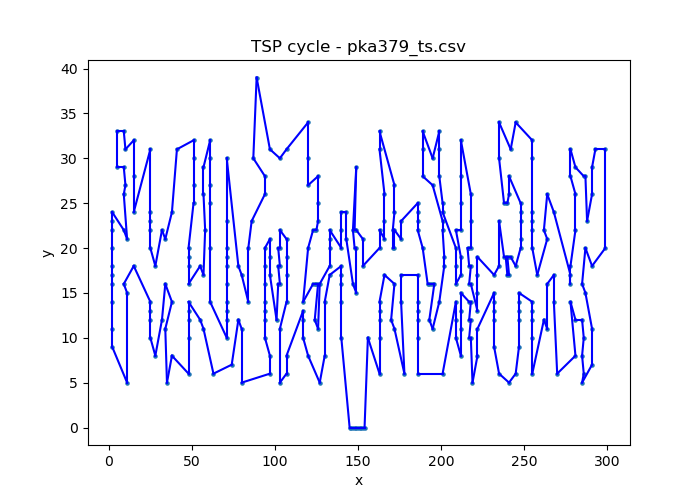
\includegraphics[width=\linewidth]{img/pka379_ts.png}
            \end{subfigure}
            \begin{subfigure}[b]{0.475\textwidth}
                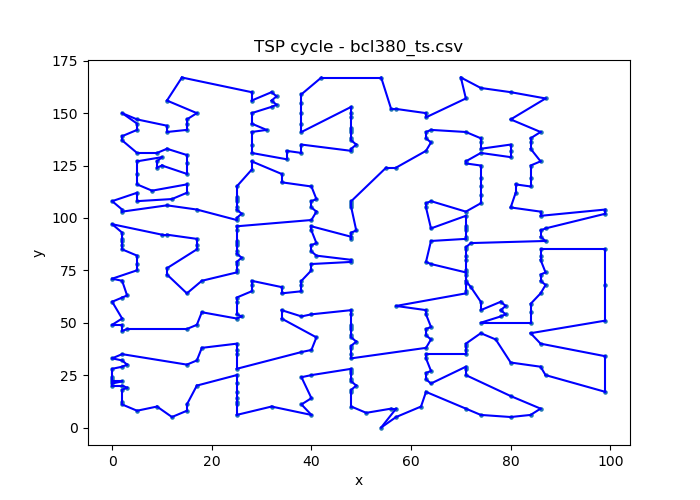
\includegraphics[width=\linewidth]{img/bcl380_ts.png}
            \end{subfigure}
            \hfill
            \begin{subfigure}[b]{0.475\textwidth}
                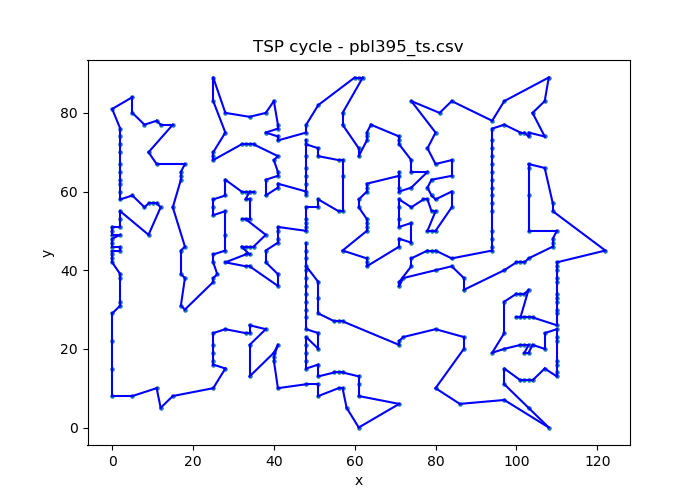
\includegraphics[width=\linewidth]{img/pbl395_ts.png}
            \end{subfigure}
            \begin{subfigure}[b]{0.475\textwidth}
                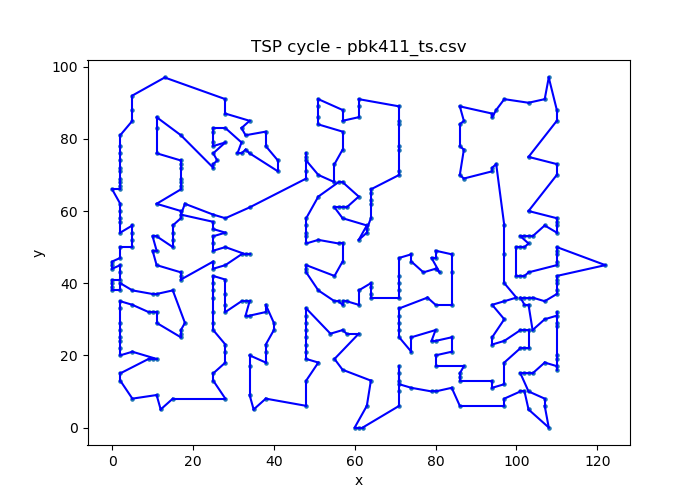
\includegraphics[width=\linewidth]{img/pbk411_ts.png}
            \end{subfigure}
            \hfill
            \begin{subfigure}[b]{0.475\textwidth}
                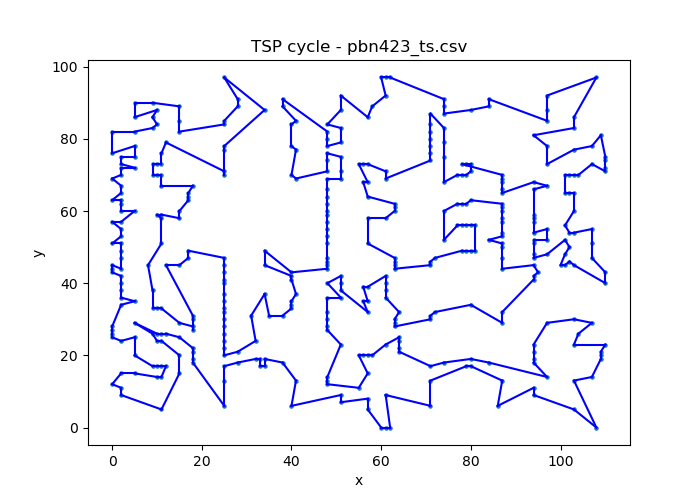
\includegraphics[width=\linewidth]{img/pbn423_ts.png}
            \end{subfigure}
            \centering
            \begin{subfigure}[b]{0.475\textwidth}
                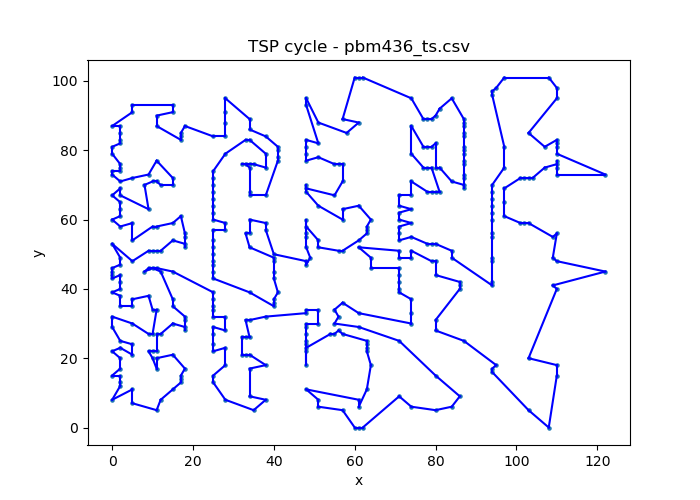
\includegraphics[width=\linewidth]{img/pbm436_ts.png}
            \end{subfigure}
            \hfill
            \begin{subfigure}[b]{0.475\textwidth}
                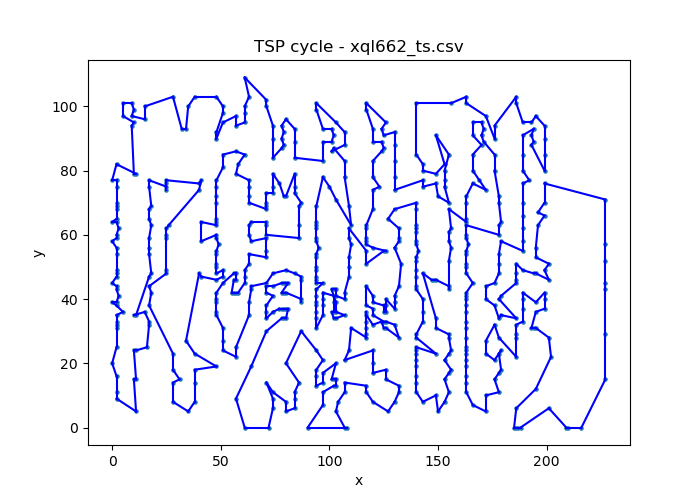
\includegraphics[width=\linewidth]{img/xql662_ts.png}
            \end{subfigure}
        \end{figure}

        \begin{figure}[htpb]
            \begin{subfigure}[b]{0.475\textwidth}
                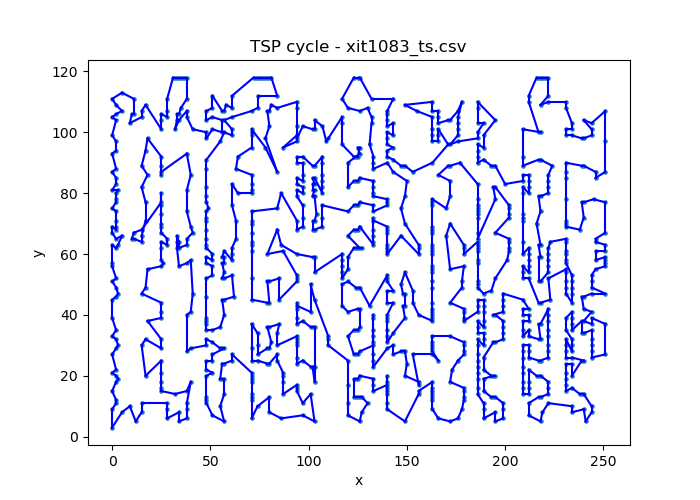
\includegraphics[width=\linewidth]{img/xit1083_ts.png}
            \end{subfigure}
            \hfill
            \begin{subfigure}[b]{0.475\textwidth}
                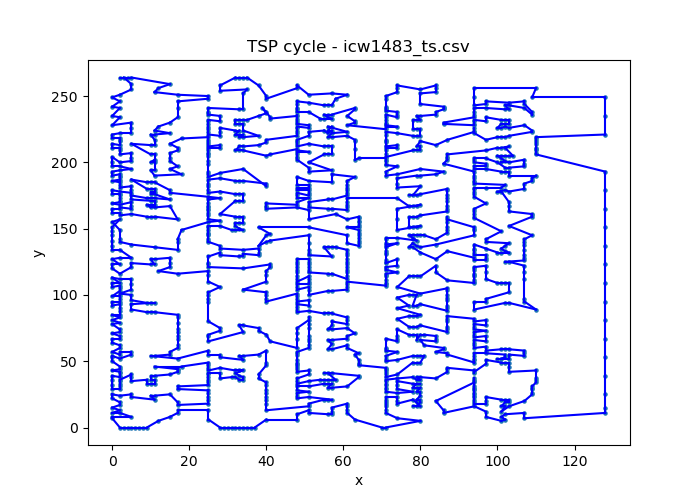
\includegraphics[width=\linewidth]{img/icw1483_ts.png}
            \end{subfigure}
            \begin{subfigure}[b]{0.475\textwidth}
                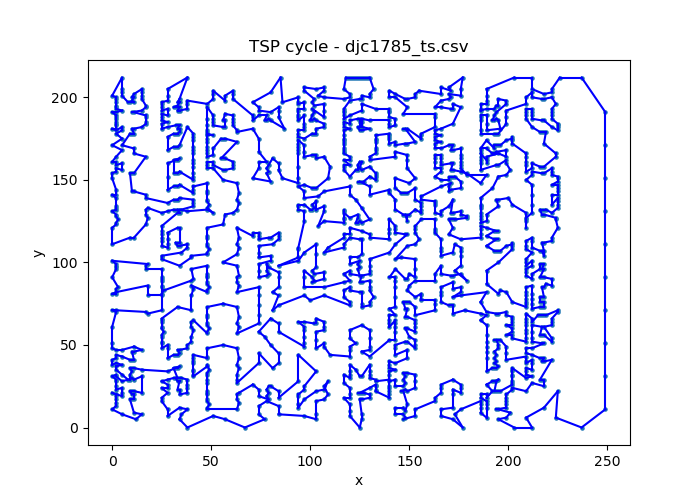
\includegraphics[width=\linewidth]{img/djc1785_ts.png}
            \end{subfigure}
            \hfill
            \begin{subfigure}[b]{0.475\textwidth}
                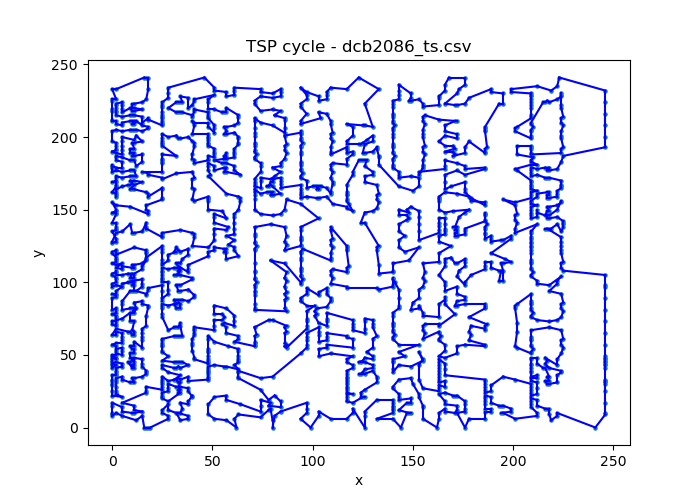
\includegraphics[width=\linewidth]{img/dcb2086_ts.png}
            \end{subfigure}
            \begin{subfigure}[b]{0.475\textwidth}
                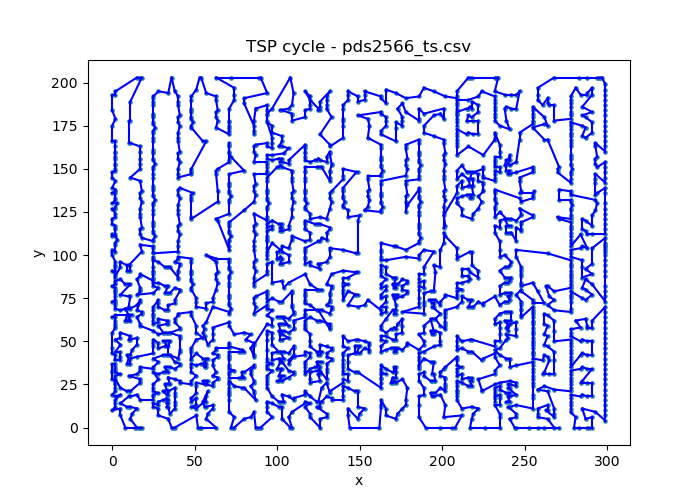
\includegraphics[width=\linewidth]{img/pds2566_ts.png}
            \end{subfigure}
            \caption{Taboo search: wizualizacja wyznaczonych cykli komiwojażera}
        \end{figure}

\end{document}
